\chapter{多维随机变量及其分布}

\intro{
	实际问题中往往需要同时考虑多个随机变量，多维随机变量的研究是概率论从一元到多元的自然推广。
}

\section{二维随机变量的分布}

\begin{mydefinition}{联合分布函数}
	设 $(X, Y)$ 为二维随机变量，\textbf{联合分布函数} $F(x, y)$ 定义为：
	\[F(x, y) = P\{X \leq x,\, Y \leq y\}.\]
\end{mydefinition}

\begin{myproperty}{矩形区域概率}
对于 $x_1 < x_2$，$y_1 < y_2$，
\[P\{x_1 < X \leq x_2,\, y_1 < Y \leq y_2\} = F(x_2, y_2) - F(x_1, y_2) - F(x_2, y_1) + F(x_1, y_1).\]
\end{myproperty}

\begin{myproperty}{联合分布函数的性质}
\begin{enumerate}
	\item 归一性：
	\[F(+\infty, +\infty) = 1,\quad F(-\infty, -\infty) = F(-\infty, y) = F(x, -\infty) = 0;\]
	\item 对每个变量单调不减；
	\item 对每个变量右连续；
	\item 矩形不等式（非负性）：对 $x_1 < x_2$，$y_1 < y_2$，
	\[F(x_2, y_2) - F(x_1, y_2) - F(x_2, y_1) + F(x_1, y_1) \geq 0.\]
\end{enumerate}
\end{myproperty}

\section{二维离散型随机变量}

\begin{mydefinition}{联合分布律}
	若 $(X, Y)$ 所有可能取值为有限对或可列无限多对，则称其为二维离散型随机变量。其联合分布律为：
	\[P\{X = x_i,\, Y = y_j\} = p_{ij}\quad (i, j = 1, 2, \ldots).\]
	满足 $p_{ij} \geq 0$ 且 $\sum_{i}\sum_{j} p_{ij} = 1$。
\end{mydefinition}

通常用分布表格表示：

\begin{center}
\begin{tabular}{c|cccc}
\toprule
$X \setminus Y$ & $y_1$     & $y_2$     & $\cdots$  & $y_j$     \\
\midrule
$x_1$ & $p_{11}$ & $p_{12}$ & $\cdots$ & $p_{1j}$ \\
$x_2$ & $p_{21}$ & $p_{22}$ & $\cdots$ & $p_{2j}$ \\
$\vdots$ & $\vdots$ & $\vdots$ & $\ddots$ & $\vdots$ \\
\bottomrule
\end{tabular}
\end{center}

\section{二维连续型随机变量}

\begin{mydefinition}{联合概率密度函数}
	若存在非负函数 $f(x, y)$，使得
	\[F(x, y) = \int_{-\infty}^{x} \int_{-\infty}^{y} f(u, v)\,du\,dv,\]
	则称 $f(x, y)$ 为 $(X, Y)$ 的\textbf{联合概率密度函数}。
\end{mydefinition}

\begin{myproperty}{联合密度函数的性质}
\begin{enumerate}
	\item 归一性：$\displaystyle\int_{-\infty}^{+\infty} \int_{-\infty}^{+\infty} f(x, y)\,dx\,dy = 1$；
	\item 密度函数与分布函数的关系：
	\[f(x, y) = \frac{\partial^2 F(x, y)}{\partial x \partial y};\]
	\item 对任意平面区域 $G \subset \R^2$，
	\[P\{(X, Y) \in G\} = \iint_G f(x, y)\,dx\,dy.\]
\end{enumerate}
\end{myproperty}

\subsection{两个常用的二维连续型分布}

\begin{mydefinition}{二维均匀分布}
	设 $D \subset \R^2$ 为有界区域，面积为 $S_D$。若
	\[f(x, y) = \begin{cases}
	\dfrac{1}{S_D}, & (x, y) \in D, \\[8pt]
	0, & (x, y) \notin D,
	\end{cases}\]
	则称 $(X, Y)$ 在 $D$ 上服从均匀分布。
\end{mydefinition}

\begin{myTheorem}{二维正态分布}
记作 $(X, Y) \sim N(\mu_1, \mu_2, \sigma_1^2, \sigma_2^2, \rho)$。
\begin{myformula}
\[
\begin{aligned}
f(x, y) = \frac{1}{2\pi\sigma_1\sigma_2\sqrt{1-\rho^2}}
\exp\biggl[-\frac{1}{2(1-\rho^2)}
\biggl(&\frac{(x-\mu_1)^2}{\sigma_1^2}
- \frac{2\rho(x-\mu_1)(y-\mu_2)}{\sigma_1\sigma_2} \\
&+ \frac{(y-\mu_2)^2}{\sigma_2^2}\biggr)\biggr].
\end{aligned}
\]
\end{myformula}

\textbf{其中：}
\begin{itemize}
	\item $\mu_1, \mu_2$：分别是 $X$ 和 $Y$ 的数学期望，决定分布中心的位置；
	\item $\sigma_1, \sigma_2$：分别是 $X$ 和 $Y$ 的标准差，决定轴向"胖瘦"；
	\item $\rho$：相关系数，反映 $X$ 和 $Y$ 之间的线性相关程度（$-1 \leq \rho \leq 1$）。
\end{itemize}
\end{myTheorem}

\begin{myproperty}{二维正态分布的重要性质}
\begin{enumerate}
	\item \textbf{边缘分布依然是正态的：} $X \sim N(\mu_1, \sigma_1^2)$，$Y \sim N(\mu_2, \sigma_2^2)$。但反之不一定成立（即边缘分布为正态，联合分布未必是正态）；
	\item \textbf{线性变换不变性：} $aX + bY \sim N(a\mu_1 + b\mu_2,\, a^2\sigma_1^2 + b^2\sigma_2^2 + 2ab\rho\sigma_1\sigma_2)$；
	\item \textbf{独立性与相关性的等价性：} 对于二维正态分布，独立与不相关（$\rho = 0$）是互为充要条件的；
	\item \textbf{等高线是椭圆：} 密度相等的点轨迹是一个椭圆，椭圆的方向和倾斜度由 $\rho$ 和 $\sigma$ 决定。
\end{enumerate}
\end{myproperty}

\begin{figure}[htbp]
\centering
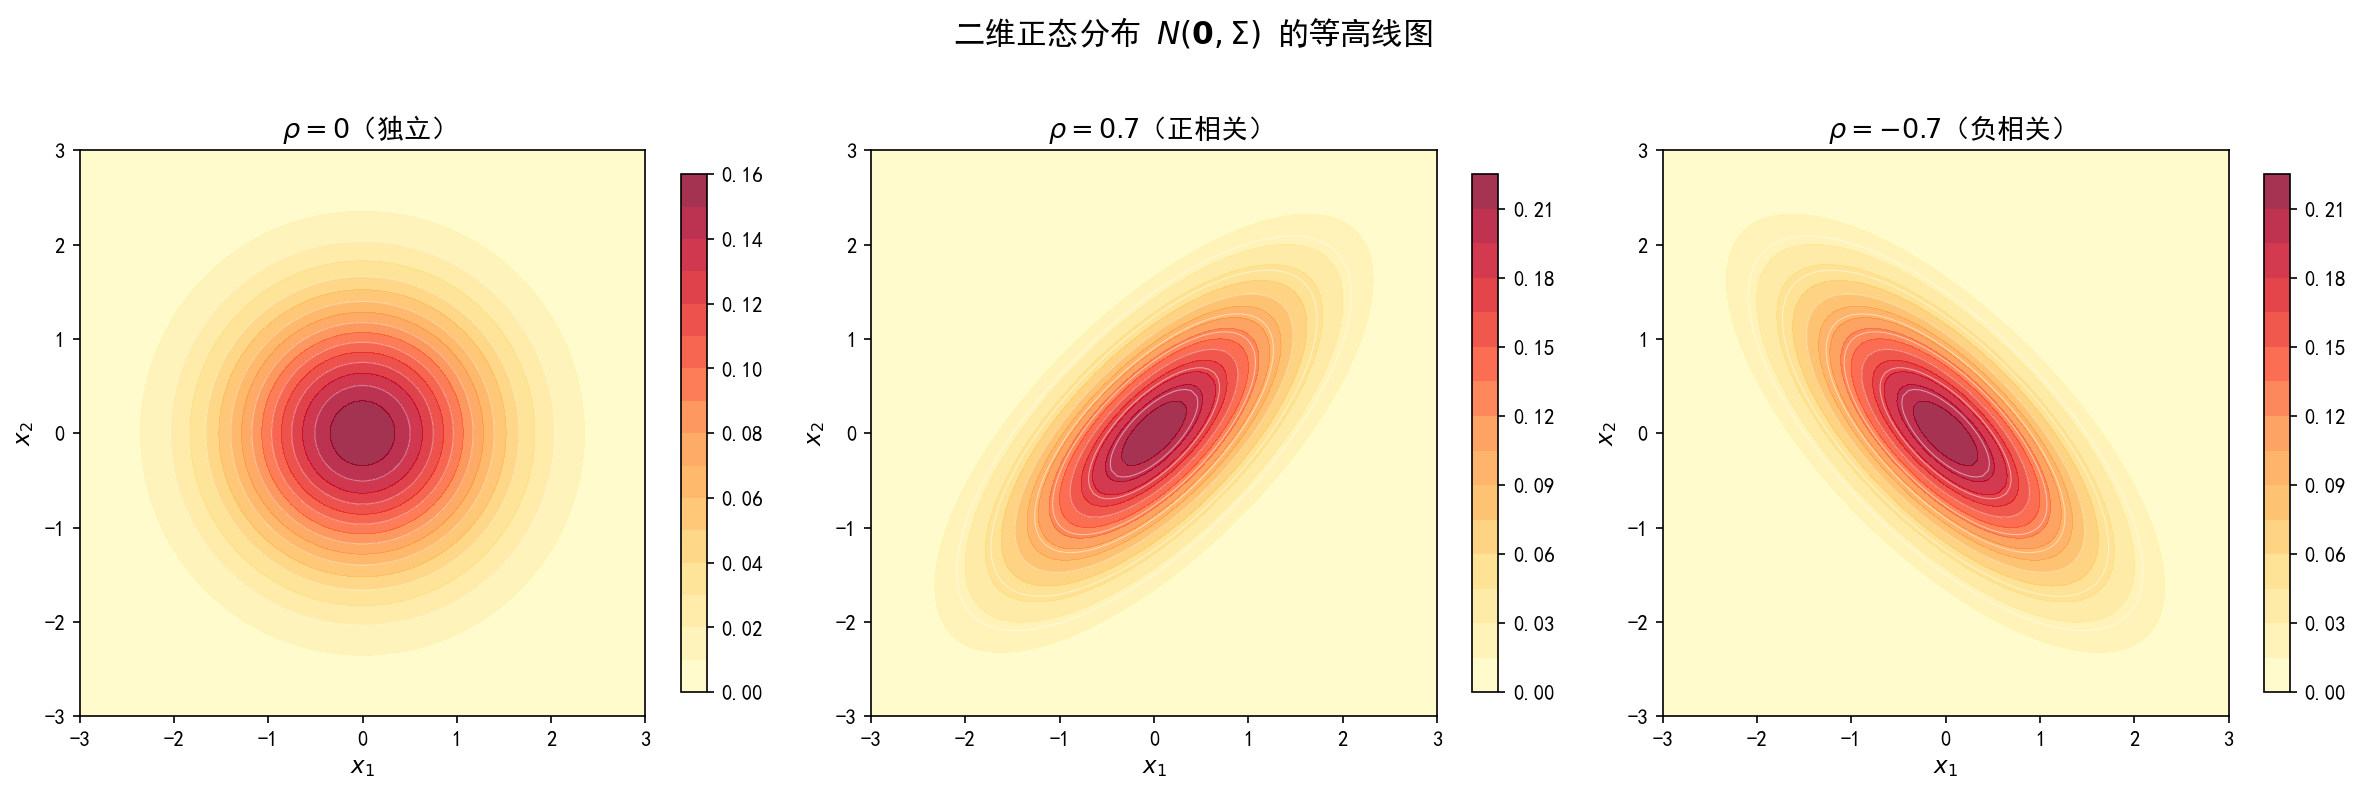
\includegraphics[width=0.6\textwidth]{Figure/bivariate_normal.png}
\caption{二维正态分布的联合概率密度曲面与等高线}
\end{figure}

\section{边缘分布}

\subsection{边缘分布函数}

从联合分布函数 $F(x, y)$ 中令另一个变量趋于无穷大，即得边缘分布函数：
\begin{myformula}
\[
\begin{aligned}
	F_X(x) &= F(x, +\infty) = \lim_{y \to +\infty} F(x, y), \\
	F_Y(y) &= F(+\infty, y) = \lim_{x \to +\infty} F(x, y).
\end{aligned}
\]
\end{myformula}

\subsection{离散型：边缘分布律}

\begin{myformula}
\[
\begin{aligned}
	P\{X = x_i\} &= \sum_{j} p_{ij} \quad\text{（行和）}, \\
	P\{Y = y_j\} &= \sum_{i} p_{ij} \quad\text{（列和）}.
\end{aligned}
\]
\end{myformula}

\subsection{连续型：边缘密度函数}

\begin{myformula}
\[
\begin{aligned}
	f_X(x) &= \int_{-\infty}^{+\infty} f(x, y)\,dy, \\
	f_Y(y) &= \int_{-\infty}^{+\infty} f(x, y)\,dx.
\end{aligned}
\]
\end{myformula}

\textbf{几何理解：} 对 $y$ 积分相当于将三维曲面沿 $y$ 方向"压扁"投影到 $x$ 轴上；对 $x$ 积分则投影到 $y$ 轴上。

\section{随机变量的独立性}

\begin{mydefinition}{独立性}
	$X$ 与 $Y$ 相互独立，当且仅当联合分布函数等于边缘分布函数的乘积：
	\[F(x, y) = F_X(x) \cdot F_Y(y).\]
\end{mydefinition}

\textbf{判定条件：}
\begin{itemize}
	\item \textbf{连续型：} $X \indep Y \iff f(x, y) = f_X(x) f_Y(y)$ 几乎处处成立；
	\item \textbf{离散型：} $X \indep Y \iff p_{ij} = p_{i\cdot} \cdot p_{\cdot j}$ 对所有 $i, j$ 成立。
\end{itemize}

\begin{theorem}[二维正态分布的独立性]
设 $(X, Y) \sim N(\mu_1, \mu_2, \sigma_1^2, \sigma_2^2, \rho)$，则
\[X \indep Y \iff \rho = 0.\]
\end{theorem}

\section{两个随机变量函数的分布}

\subsection{离散型情形}

设 $Z = g(X, Y)$，其分布律为：
\[P\{Z = z_k\} = \sum_{g(x_i, y_j) = z_k} P\{X = x_i,\, Y = y_j\}.\]

\begin{myTheorem}{和的分布}
$Z = X + Y$。
\[P\{Z = z\} = \sum_i P\{X = x_i,\, Y = z - x_i\}.\]
若 $X \indep Y$，则为\textbf{离散卷积}：
\[P\{Z = z\} = \sum_i P\{X = x_i\} \cdot P\{Y = z - x_i\}.\]
\end{myTheorem}

\begin{myTheorem}{最值分布}
设 $X_1, \ldots, X_n$ 相互独立，分布函数分别为 $F_1, \ldots, F_n$，则
\begin{myformula}
\[
\begin{aligned}
    F_M(z) &= F_1(z) F_2(z) \cdots F_n(z), \\
    F_N(z) &= 1 - [1 - F_1(z)] [1 - F_2(z)] \cdots [1 - F_n(z)].
\end{aligned}
\]
\end{myformula}
其中 $M = \max\{X_1, \ldots, X_n\}$，$N = \min\{X_1, \ldots, X_n\}$。
\end{myTheorem}

\subsection{连续型情形}

\begin{myTheorem}{分布函数法（通用方法）}
设 $Z = g(X, Y)$：
\begin{enumerate}
	\item 先求 CDF：$\displaystyle F_Z(z) = P\{g(X, Y) \leq z\} = \iint_{g(x, y) \leq z} f(x, y)\,dx\,dy$；
	\item 求导得 PDF：$f_Z(z) = \dfrac{d}{dz} F_Z(z)$。
\end{enumerate}
关键在于确定积分区域 $D_z = \{(x, y) \mid g(x, y) \leq z\}$。
\end{myTheorem}

\begin{myTheorem}{变量代换法（Jacobi 行列式法）}
设变换 $u = g_1(x, y)$，$v = g_2(x, y)$，逆变换 $x = h_1(u, v)$，$y = h_2(u, v)$，则
\[f_{U,V}(u, v) = f_{X,Y}\bigl(h_1(u, v), h_2(u, v)\bigr) \cdot \abs{J},\]
其中 Jacobi 行列式：
\begin{myformula}
\boxed{\displaystyle J = \frac{\partial(x, y)}{\partial(u, v)} = \det\begin{pmatrix}
\dfrac{\partial x}{\partial u} & \dfrac{\partial x}{\partial v} \\[8pt]
\dfrac{\partial y}{\partial u} & \dfrac{\partial y}{\partial v}
\end{pmatrix}.}
\end{myformula}

最后通常需要对 $v$ 求边缘分布来得到 $U$ 的密度：$f_U(u) = \int_{-\infty}^{+\infty} f_{U,V}(u, v)\,dv$。
\end{myTheorem}

\subsection{常见函数的密度公式}

\begin{myTheorem}{和的分布（卷积公式）}
$Z = X + Y$，$X \indep Y$。
\begin{myformula}
\boxed{\displaystyle f_Z(z) = \int_{-\infty}^{+\infty} f_X(x) f_Y(z - x)\,dx.}
\end{myformula}
\end{myTheorem}

\begin{myTheorem}{商的分布}
$Z = Y / X$，$X \indep Y$，$X > 0$。
\[f_Z(z) = \int_{0}^{+\infty} x f_X(x) f_Y(zx)\,dx.\]
\end{myTheorem}

\begin{myTheorem}{正态分布的可加性}
若 $X \sim N(\mu_1, \sigma_1^2)$，$Y \sim N(\mu_2, \sigma_2^2)$ 且独立，则
\[X \pm Y \sim N(\mu_1 \pm \mu_2,\, \sigma_1^2 + \sigma_2^2).\]
更一般地，独立正态随机变量的线性组合仍服从正态分布。
\end{myTheorem}
